\chapter{Characterization}
\label{chap:Char}
The goal of the work is to characterize the energy and latency of end-to-end ODS camera  systems and propose optimizations. As the existing ODS camera systems are built from off the shelf camera devices and use the conventional stitching algorithms, they capture redundant data and perform redundant computations. The main challenge in ODS panorama generation is to understand the data flow across the system and to make decisions on data abstractions needed at different subcomponents to reduce the total system power and latency.

We classify our findings into two categories, i.e the reasons for high energy and high latency.
For high energy or power consumption, we divide into following three categories
\begin{itemize}
	\item Redundant Capture, and Computations
	\item High Data rates across interfaces
	\item Huge memory footprint
\end{itemize}
For high latency we analyze,
\begin{itemize}
	\item Effect of sequential execution on stage and sub-stage latencies.
\end{itemize}

\section{Measurement Methodology} % Energy and Latency Measurement 
Jetson has INA3221 monitors and I2C capabilities to read voltage, current and power for different rails on the SOC and IO. For evaluation we measure the absolute energy of the system and the difference between the idle and active state for individual stages of the pipeline. We also use NVIDIA Tegra stats command to check the clock frequencies of different components like CPU, GPU, Memory Controller for validation. 

The latency of the camera capture and ISP is defined by the framerate (i.e throughput), where for computation stages we measure the latencies in terms of CPU runtime of individual software components in the stitching pipeline. One of the critical components of stitching pipeline is optical flow which can take several seconds to compute each output frame on low power embedded CPU. Therefore for realistic estimation of optical flow for accelerator based design, we measure the power and latency of optical flow implementation on Zynq FPGA board. 

\section{Energy Characterization}
We first highlight the overall system energy profile. For the calculating the energy for frame in the above table, the camera capture is configured to 1920x1080 resolution at 30 fps, and the output resolution is 3k. We then explain about the key findings discussed in the introduction of this chapter. 
\subsubsection{Individual stage energy}

\begin{table}[h]
		\\\specialrule{3pt}{0pt}{0pt}
	\begin{tabular}
		{!{\VRule[2pt]}c|!{\VRule[2pt]}c!{\VRule[2pt]}c!{\VRule[2pt]}c!{\VRule[2pt]}}
	Subsystem & Current(mA) & Voltage(mV) & Energy( mJ/frame) \\\specialrule{2pt}{0pt}{0pt}
	Sony IMX-274 (Camera) & 375.4 & 3336 & 41.7 \\\hdashline
	ISP+CODEC (TX2) & 102.7 & 19152 & 65.6 	\\\hdashline
	ARM-A57(Cap. + Stitch*) & 16.4 + 120* & 19144 & 10.5 + 36,736	\\\hdashline
	DRAM (Cap. + Stitch*)  & 260.4 + 105*  & 4792 & 41.6 + 1680 	\\\specialrule{2pt}{0pt}{0pt}
	\end{tabular} 
	\caption{Energy Characterization of Individual Stages}
\label{Tab:Energy_Char}
\end{table}

	Note*: As seen in the above table \ref{Tab:Energy_Char}, the stitching in software is highly expensive for CPU,and DRAM blocks, i.e the computation stage energy dominates the capture stage. CPU runtime to render each output frame of 3k is ~16 sec, which increases the both the energy and end-to-end latency. The other options include using GPU's, FPGA, ASIC's. Therefore, we approximate the energy and latency for FPGA based accelerator based on Xilinx's implementation of optical flow on Zynq board, discussed in chapter5.\newline

\subsubsection{Redundant Capture}
Natural images are redundant and but sensors are not smart to capture only the variations of the scene. Instead sensors capture and convert all the pixels for all the temporal frames. This leads to redundant conversion cycles by ADC's inside the sensor. It is therefore important to reuse the previous data to reduce the conversion cycles of the ADC to reduce the sensor power. 
\begin{figure}[h]
	\begin{center}
		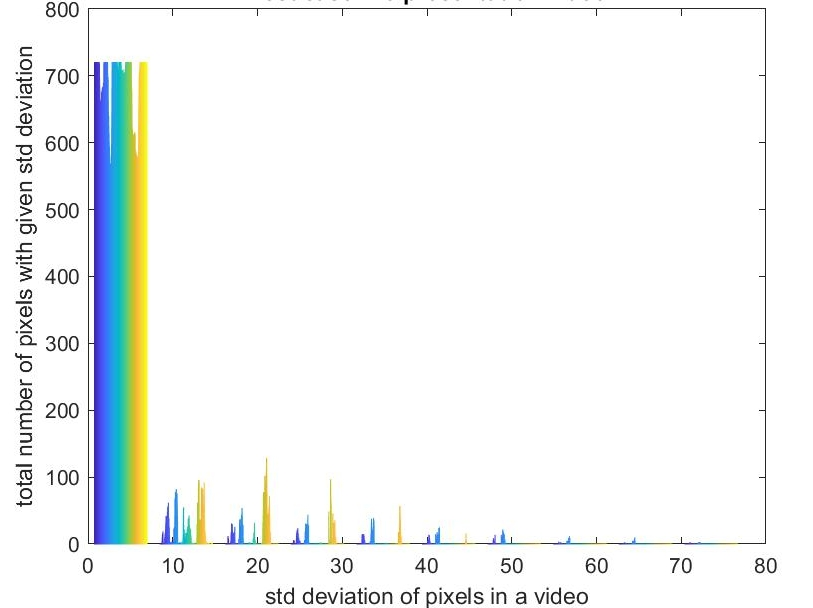
\includegraphics[width=1\textwidth]{data/images/Best_case_rio_presentation.jpg}
	\end{center}
	\caption{X axis shows the variations of pixels across 1000 consecutive frames, Y axis shows total number of pixels with a particular variation}	
	\label{fig:sensorRedundancy}
\end{figure} 

\subsubsection{High Data rates across interfaces}
As shown in the \ref{fig:pieCapPow}, the interfaces consume about one third of total power during capture. The high data rates lead lead to higher power consumption. But having compression near sensor and decompression near ISP will increase to high latency and may increase the sub-system power. A neat technique is to use the co-design of ISP with the interface encoding schemes. The ISP has Bayer statistics for different regions of the image. As the temporal frames are redundant, the Bayer statistics can be used for encoding CSI interface data efficiently. 

\begin{figure}[h]
	\begin{center}
		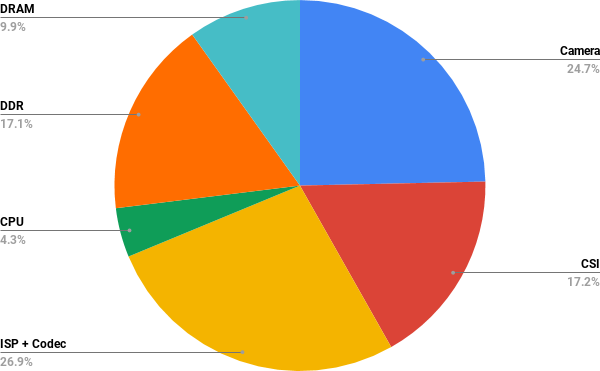
\includegraphics[width=1\textwidth]{data/images/chart.png}
	\end{center}
	\caption{Chart showing the distribution of power of different components during capture and storage.}	
	\label{fig:pieCapPow}
\end{figure} 

\subsubsection{Huge Memory Footprint}
The existing offloading based solutions have high memory footprint. One of the main reason being the inability to reuse the data generated by different subsystems. For example, during optical flow we load the current and previous image frames just to compute motion vector data. But this data is already available in ISP stage. Having data abstractions to reuse such data can reduce the memory requirement by up to 50 \%.


\subsubsection{Redundant Computations}
Similar to the sensor capture, the stitching algorithms perform lot of redundant memory access and computations. Even though only few pixels change between frames, the existing algorithms compute over the entire image for every frame. Building custom hardware with fine power gating can be used to reduce the activity of the computation units where the there is no motion across frames. 



\section{Latency Characterization}

\subsubsection{Individual Stage latency}


For camera system and ISP stages the stage latency is derived from throughput, i.e inverse of fps. The end to end latency is as given in NVIDIA camera API documentation, which is one frame latency for camera stage, and one for ISP stage. 

We measure the latency of computation in terms of CPU runtime. The optical flow, view synthesis and image sharpening stages take 98\% of total CPU runtime. The CPU  implementation takes 24 seconds for generating output at 6k resolution, of which optical flow generation consumes nearly 70 \% of runtime. We therefore focus on reducing the optical flow stage which dominates not just in terms of latency but also in power consumption. 


\subsubsection{Optical flow runtime breakdown}
The individual stages and the sub-stages of computation are sequential, leading to higher runtimes. By pipelining the different pyramid computation stages of optical flow, we can reduce the latency to 0.1 seconds from 16 seconds as shown in \ref{fig:OF_pyr_runtime}.

\begin{figure}[h]
	\begin{center}
		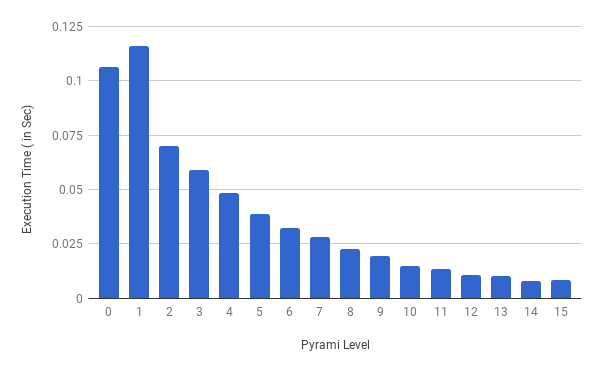
\includegraphics[width=1\textwidth]{data/images/pyramid_runtime.png}

	\end{center}
		\caption{X-axis shows the pyramid level and Y-axis shows the runtime for OF}
\label{fig:OF_pyr_runtime}
\end{figure} 

\section{Design Scalability}	

\subsubsection{Runtime scalability with the resolution}
As discussed in chapter 2 related work, the resolution required for next generation VR is at-least 16k and frame-rates greater than 120. For our evaluation, we assume that energy scales linear with frame-rate and focus our evaluation on scalability of increasing resolution. We can see in fig that even the runtime scales almost linearly with the resolution. Notice that optical flow dominates the total runtime, followed by view synthesis and image sharpening. We also measure the frequencies of CPU, DRAM controller with increasing resolution and observe [linear] dependency of clock frequency on the resolution.
\begin{figure}[h]
	\begin{center}
		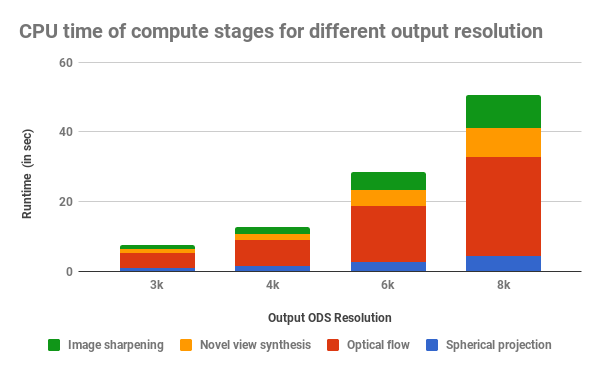
\includegraphics[width=1\textwidth]{data/images/ExecutionTimeComputeStages.png}
		\caption{CPU execution time of different compute stages. X axis has different sub-stages in optical flow and Y axis correspond to energy per frame.}
		\label{fig:ex_4_9}
	\end{center}
	\vspace{-0.3in}
\end{figure} 

The main takeaway is that the existing hardware and software scale linearly with the increasing resolution and framerate, which is bad considering the VR panorama requirements. We therefore propose directions to exploit the spatio-temporal redundancies within the frame and across the frames to reduce the data flow and computation. We propose rasterbuffer based design to decrease the chip resources, and use data abstractions at different hardware IP blocks to share data to reduce temporal redundancies(eg. motion vectors from ISP can be used by optical flow stage, thereby removing the necessity to store previous frames and recomputation of motion data at a later time. The same motion vectors can be used to encode spatial frame data to reduce redundant data transfer).
%What is the energy per each output pixel	
%What is energy per pixel when generating only one ODS view, and how does it compare when generating two views! If it is double then we have a problem to solve	
%[Check why sharpening is so costly!]

\subsubsection{Resource scalability with the resolution}
We measure the DRAM capacity and bandwidth needs as we increase the resolution as a parameter for resource scalability. Higher capacity indicates the need for better encoding schemes and high bandwidth can indicate the temporal redundancy in the data, thereby increasing the bandwidth requirement. For 3k, 4k, 6k and 8k output resolution.

Although we built a system where all the cameras are capturing at same resolution and framerate at a given time, we expect the future cameras make these decisions dynamically to save power. Therefore, we  measure the efficiency of capture and ISP processing at different modes of operation and measure the efficiency of capture and processing in power consumed per pixel at different modes.

% Figure 
\begin{figure*}
	\begin{center}
		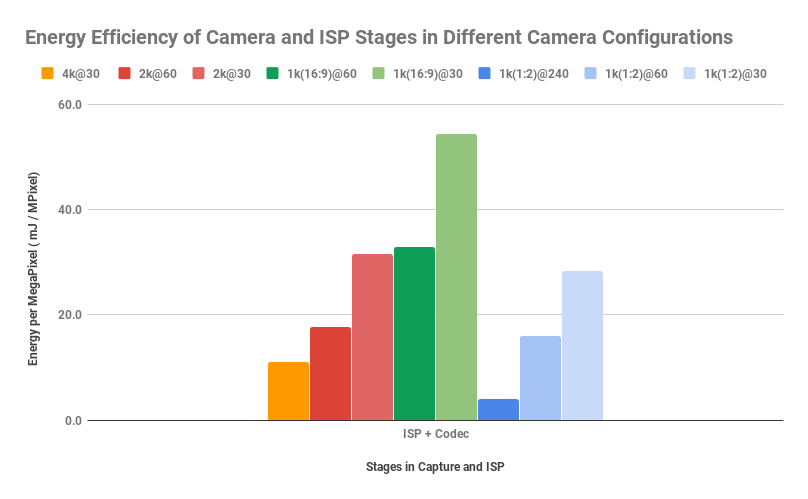
\includegraphics[width=1\textwidth]{data/images/EnergyEfficiencyofCameraandISPStagesinDifferentCameraConfigurations}
		\caption{Energy Efficiency of Camera ISP Stages in different configurations}
		\label{fig:ex_4_9}
	\end{center}
\end{figure*} 



\section{Different sensor configurations for energy efficiency and quality}
\subsubsection{Saving sensor power}
As the ODS consist of several cameras, it makes sense to reconfigure or turn cameras or off based on the application needs and the scene dynamics. If the camera is not moving and certain portions of the camera views are static, the cameras can be reconfigured dynamically to reduce framerate, resolution, or even turn them on and off as per the needs. We observed that the reconfiguration latency is one frame delay if there are no outstanding requests, and if there are pending camera requests, they will be served first before requesting the frame with new configuration. 
\subsubsection{Improving quality of images in low lighting}
The optical flow works well when the image is has high dynamic range. It is possible that some of the regions in the 360 degree view can be in low lightning, while other are in good lightning conditions. In such cases the stitching fails and can have severe artifacts. We can improve the dynamic range of the particular cameras in low lightning by reconfiguring the camera exposure time dynamically. But such approaches do not consider the end to end latency of the cameras and camera movements. To account for camera movements, IMU sensor data can be used to make the camera configuration decisions independent of CPU to accelerate the reconfiguration tasks. 

The figures \ref{fig:histLow} and  \ref{fig:histHigh} show the differences in low light capture with and without brightness correction.
	\begin{figure}[h]
	\begin{center}
		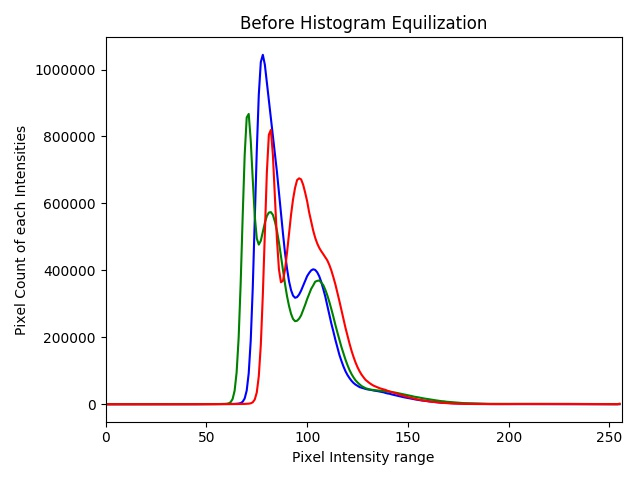
\includegraphics[width=0.8\textwidth]{data/images/Before_Histogram_equilization.jpg}
		\caption{Image intensity histogram for low lightning conditions}
		\label{fig:histLow}
	\end{center}
	\vspace{-0.3in}
\end{figure} 

\begin{figure}[h]
	\begin{center}
		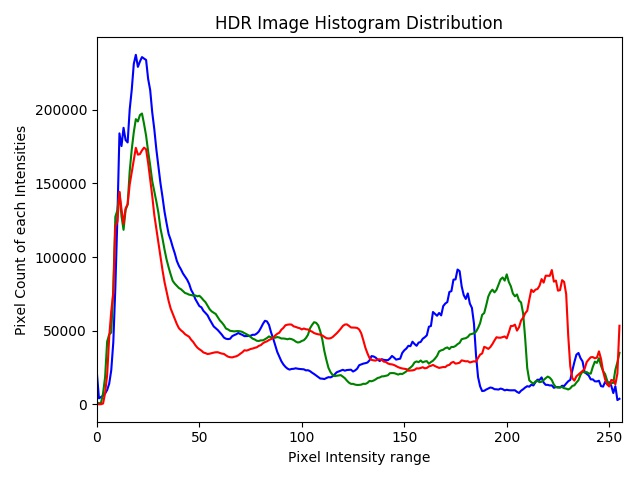
\includegraphics[width=0.8\textwidth]{data/images/Normal_Histogram_Distribution.jpeg}
		\caption{Image intensity histogram for good lightning conditions}
		\label{fig:histHigh}
	\end{center}
	\vspace{-0.3in}
\end{figure} 

